% !TeX encoding = UTF-8
% !TeX spellcheck = ru_RU
\documentclass[a4paper,14pt]{extarticle} %размер бумаги устанавливаем А4, шрифт 14пунктов
\usepackage{amssymb,amsfonts,amsmath,mathtext,cite,enumerate,float} %подключаем нужные пакеты расширений
\usepackage[T2A, T1]{fontenc}
\usepackage{cmap}
\usepackage[utf8]{inputenc}%включаем свою кодировку: koi8-r или utf8 в UNIX, cp1251 в Windows
\usepackage[english, russian]{babel}%используем русский и английский языки с переносами

\usepackage{graphicx} %хотим вставлять в диплом рисунки?
\graphicspath{{img/}}%путь к рисункам

\usepackage[colorlinks=false,pdfborder={0 0 0}]{hyperref} %использование гиперссылок, colorlinks - цвет текста ссылки, pdfborder - окантовка. 

%шрифт Times New Roman
%\usepackage{fontspec}
%\setmainfont{Times New Roman}
%\setallmainfonts{Times New Roman}

\usepackage{titlesec}
\titleformat{\section}[block]
{\filcenter\large}
{\thesection}
{1em}{\MakeUppercase}
\titlespacing*{\section}{0pt}{-30pt}{*4}

\makeatletter
%\renewcommand{\@biblabel}[1]{#1.} % Заменяем библиографию с квадратных скобок на точку:
\makeatother


\usepackage{geometry} % Меняем поля страницы
\geometry{left=3cm}% левое поле
\geometry{right=15mm}% правое поле
\geometry{top=2cm}% верхнее поле
\geometry{bottom=2cm}% нижнее поле
\linespread{1.5}

\usepackage{indentfirst} % отделять первую строку раздела абзацным отступом
\setlength\parindent{5ex}

%links
\usepackage{url}

\usepackage[tableposition=top,singlelinecheck=false, justification=centering]{caption}
\usepackage{subcaption}

%  маркированные списки
\renewcommand{\labelitemi}{--}
\renewcommand{\labelitemii}{--}
%  нумерованные списки
\renewcommand{\labelenumi}{\asbuk{enumi})}
\renewcommand{\labelenumii}{\arabic{enumii})}

% номер сноски со скобкой
\renewcommand*{\thefootnote}{\arabic{footnote})}
\renewcommand{\footnoterule}{%
	\kern -3pt
	\hrule width 40mm height .4pt
	\kern 2.6pt
}

%иллюстрации и таблицы
\DeclareCaptionLabelFormat{gostfigure}{Рисунок #2}
\DeclareCaptionLabelFormat{gosttable}{Таблица #2}
\DeclareCaptionLabelSeparator{gost}{~---~}
\captionsetup{labelsep=gost}
\captionsetup*[figure]{labelformat=gostfigure}
\captionsetup*[table]{labelformat=gosttable}
\renewcommand{\thesubfigure}{\asbuk{subfigure}}


%\renewcommand{\rmdefault}{ftm}
\renewcommand{\figurename}{Рисунок} % Рис -> Рисунок
%\usepackage[labelsep=period,labelfont=bf,figurename={Рисунок},figurewithin=none]{caption}
\renewcommand{\theenumi}{\arabic{enumi}}% Меняем везде перечисления на цифра.цифра
\renewcommand{\labelenumi}{\arabic{enumi}}% Меняем везде перечисления на цифра.цифра
\renewcommand{\theenumii}{.\arabic{enumii}}% Меняем везде перечисления на цифра.цифра
\renewcommand{\labelenumii}{\arabic{enumi}.\arabic{enumii}.}% Меняем везде перечисления на цифра.цифра
\renewcommand{\theenumiii}{.\arabic{enumiii}}% Меняем везде перечисления на цифра.цифра
\renewcommand{\labelenumiii}{\arabic{enumi}.\arabic{enumii}.\arabic{enumiii}.}% Меняем везде перечисления на цифра.цифра

\usepackage{tocloft}
\renewcommand{\cftsecleader}{\cftdotfill{\cftdotsep}}
%\renewcommand{\cfttoctitlefont}{\Large\filcenter}

%\setcounter{page}{2} %нумерация страниц с 3
%\addto\captionsrussian{\renewcommand\contentsname{СОДЕРЖАНИЕ}}
%\addto\captionsrussian{\renewcommand\refname{СПИСОК ИСПОЛЬЗОВАНЫХ ИСТОЧНИКОВ}}

\usepackage{listings}

\begin{document}
	% !TeX spellcheck = ru_RU
% !TeX encoding = UTF-8
\section{Общая структурная схема и план описания системы}
\subsubsection{Общая структурная схема}\label{7.1}
В данном подразделе мы рассмотрим общую структурную схему системы. Данная общая схема отражает основные особенности реальных систем, которые будут рассмотрены в последующих разделах.
Общая структурная схема системы представлена на рисунке 
\ref{fig:common_chart}.

\begin{figure}[H]
	\centering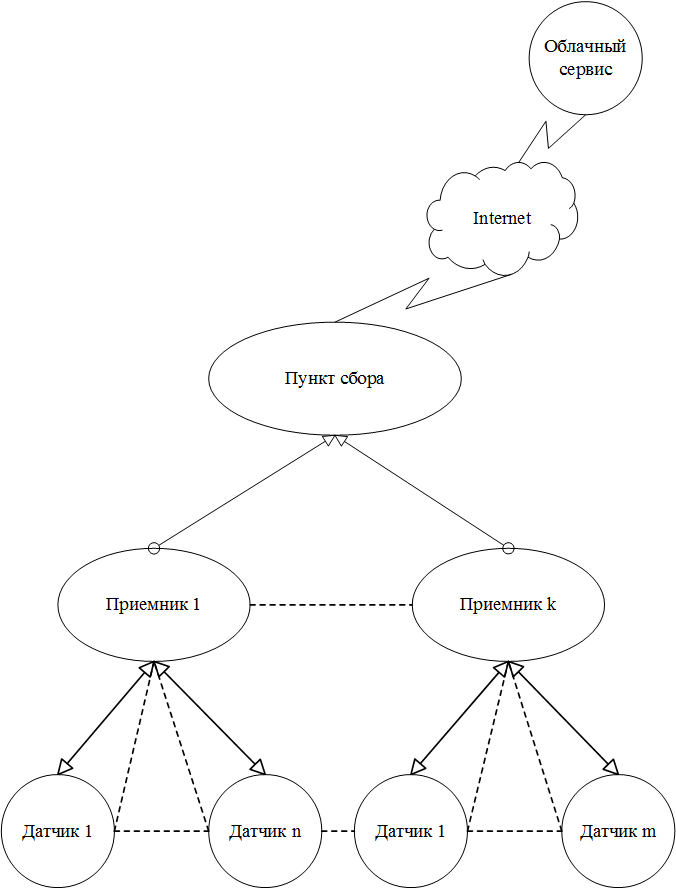
\includegraphics[width=0.7\linewidth]{img/common_chart}
	\caption{Общая структурная схема системы}
	\label{fig:common_chart}
\end{figure}

В системе имеются следующие компоненты: 
\begin{itemize}
	\item "Датчики".
	\item "Приёмники". 
	\item "Пункт сбора".
	\item Облачный сервер.
\end{itemize}

Под "датчиком" будем понимать устройство, которое включает в себя некоторый сенсор (например, термо-датчик, датчик освещенности и т.п.) и передающее устройство. В некоторых случаях "датчик" может содержать не только передающее, но и принимающее устройство. Кроме того, иногда "датчик" может содержать не только сенсор, но и некоторый исполнительный механизм (например, сервопривод). Под "приёмником" будем понимать устройство, которое принимает данные от нескольких "датчиков", делает некоторую обработку и передает эти данные далее на "пункт сбора". В некоторых случаях "приёмник" может принимать данные от "пункта сбора" и передавать их "датчикам".

В общем случае работу системы можно описать следующим образом. Данные от "датчиков" по определенному протоколу передаются "приёмником".
На одном "приёмнике" принимаются данные от нескольких "датчиков" и предварительно обрабатываются. Данные от "приёмников" по определенному протоколу передаются на "пункт сбора", где производится дальнейшая обработка этих данных. С "пункта сбора" данные по протоколу TCP/IP или UDP/IP через интернет передаются в некоторый облачный сервер.

В некоторых случаях от "пункта сбора" на "приёмник" могут передаваться данные, которые далее "приёмник" передает на "датчики"(например, это управляющие команды, которые производят настройку сенсоров и т.п).  
\subsubsection{План описания системы}
Каждую систему будем описывать по следующему плану:
\begin{itemize}
	\item Назначение системы.
	\item Структура системы. 
	\item Разбиение системы на уровни.
	\item Особенности построения уровней.
\end{itemize}
При описании назначения системы необходимо указать область применения данной системы, частотный радиодиапазон, в котором работает система, стандарты, на основе которых построена данная система и т.п. Кроме того, при описании назначения системы, необходимо дать ссылки на источники, где описана данная система. 

Рассказывая о структуре системы необходимо показать, как соотносится структура системы с общей структурной схемой системы,
описанной в разделе \ref{7.1}.
и указать, возможна ли в данной системе передача данных от "приемников" к "датчикам".    

Описывая  разбиение системы на уровни, необходимо дать краткое описание каждого уровня и указать, является ли данный уровень открытым или нет.

Если у системы есть специфические особенности построения некоторых уровней, то их необходимо описать и дать ссылки на источники, где имеется подробное описание этих особенностей.
\newpage
	% !TeX spellcheck = ru_RU
% !TeX encoding = UTF-8
\section{Технология Lora}
\subsubsection{Назначение}
Технология LoRa включает в себя метод модуляции LoRa, разработанный Semtech, и открытый протокол LoRaWAN.

Если модуляция LoRa является физическим уровнем (OSI media layer 1), то LoRaWAN (Long Range Wide-Area Networks) – это MAC протокол канального уровня (OSI media layer 2) для сетей с множеством узлов с большим радиусом действия и низким собственным потреблением мощности.   

Узлам сети характерны: низкое энергопотребление (до 10 лет работы от обычных батарей АА), невысокая скорость обмена данными, большая дальность связи (15 км в сельской местности и 5км в плотной городской застройке) и низкая стоимость оконечного оборудования.

Разработчики LoRa Alliance позиционируют LoRa как технологию, имеющую значительные преимущества перед сотовыми сетями и WiFi благодаря возможности развертывания межмашинных (M2M) коммуникаций на расстояниях до 15 км и скоростях до 50 Кбит/с, при минимальном потреблении электроэнергии, обеспечивающем несколько лет автономной работы на одном аккумуляторе типа АА.

Диапазон применений данной технологии огромен: от домашней автоматизации и интернета вещей (Internet of Things, IoT) до промышленности и умных городов.

\subsubsection{Структура системы}
Рассмотрим структуру LoRaWAN сетей. Типичная сеть LoRaWAN состоит из следующих элементов: 
\begin{itemize}
	\item"Датчики". В технологии LoRa используется термин "конечные узлы".
	\item"Приёмники". В технологии LoRa используется термин "шлюзы".
	\item"Пункт сбора". В технологии LoRa используется термин "сетевой сервер".
	\item"Облачный сервер". В технологии LoRa используется термин "сервер приложений".
\end{itemize}

Структурная схема системы представлена на рисунке
\ref{fig:LoRa}.
\begin{figure}[H]
	\centering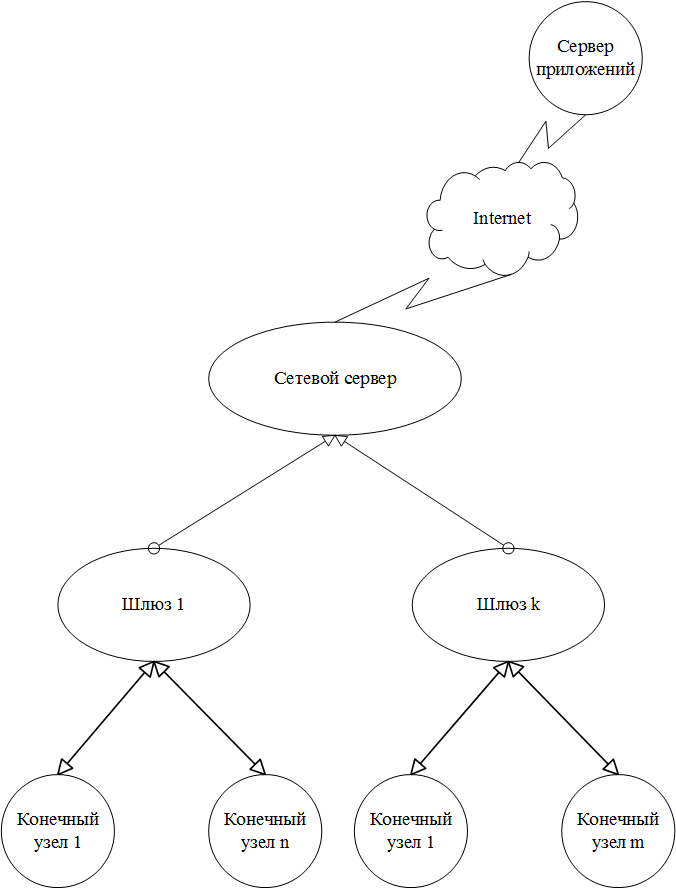
\includegraphics[width=0.7\linewidth]{img/LoRa}
	\caption{Структурная схема системы, построенной по технологии LoRa}
	\label{fig:LoRa}
\end{figure}


\textbf{Конечный узел (End Node) }предназначен для осуществления управляющих или измерительных функций. Он содержит набор необходимых датчиков и управляющих элементов.

\textbf{Шлюз LoRa (Gateway/Concentrator)} — устройство, принимающее данные от конечных устройств с помощью радиоканала и передающее их в транзитную сеть. В качестве такой сети могут выступать Ethernet, WiFi, сотовые сети и любые другие телекоммуникационные каналы. Шлюз и конечные устройства образуют сетевую топологию типа звезда. Обычно данное устройство содержит многоканальные приёмопередатчики для обработки сигналов в нескольких каналах одновременно, или даже нескольких сигналов в одном канале. Соответственно, несколько таких устройств обеспечивает зону покрытия сети и прозрачную двунаправленную передачу данных между конечными узлами и сервером.

\textbf{Сетевой сервер (Network Server)} предназначен для управления сетью: заданием расписания, адаптацией скорости, хранением и обработкой принимаемых данных.

\textbf{Сервер приложений (Application Server)} может удаленно контролировать работу конечных узлов и собирать необходимые данные с них \cite{1}.

В конечном итоге, LoRaWAN сеть имеет топологию звезда, имеет конечные узлы, которые через шлюзы, образующие прозрачные мосты, общаются с центральным сервером сети. При таком подходе обычно предполагается, что шлюзами и центральным сервером владеет оператор сети, а конечными узлами – абоненты. Абоненты имеют возможность прозрачной двунаправленной и защищенной передачи данных до конечных узлов.

Так как LoRaWAN образуют глобальную сеть, то разработчики уделили особое внимание безопасности и конфиденциальности передаваемых данных, которые обеспечиваются шифрованием AES на нескольких уровнях:



\begin{itemize}
	\item На сетевом уровне с использованием уникального ключа сети (Unique Network key, EUI64).
	\item Сквозную безопасность на уровне приложений с помощью уникального ключа приложения (Unique Application key, EUI64).
	\item И специального ключа устройства (Device specific key, EUI128).
\end{itemize}

Для решения различных задач и применений в сети LoRaWAN предусмотрено три класса устройств:

1. Двунаправленные конечные устройства «класса А» (Bi-directional end-devices, Class A). Устройства этого класса применяются, когда необходима минимальная потребляемая мощность при преобладании передачи данных к серверу. В качестве инициатора сеанса связи выступает конечный узел, отправляя пакет с необходимыми данными, а затем выделяет два окна, в течении которых ждёт данных от сервера. Таким образом, передача данных от сервера возможна только после выхода на связь конечного устройства.

2. Двунаправленные конечные устройства «класса Б» (Bi-directional end-devices, Class B). Основное отличие от устройств «класса А» заключается в выделении дополнительного окна приёма, которое устройство открывает по расписанию. Для составления расписания конечное устройство осуществляет синхронизацию по специальному сигналу от шлюза. Благодаря этому дополнительному окну сервер имеет возможность начать передачу данных в заранее известное время.

3. Двунаправленные конечные устройства «класса С» с максимальным приемным окном (Bi-directional end-devices, Class C). Устройства этого класса имеют почти непрерывное окно приёма данных и закрывают его лишь на время передачи данных, что позволяет их применять для решения задач, требующих получения большого объёма данных.

Подводя итоги, можно сказать, что LoRaWAN позволяет строить глобальные распределённые беспроводные сети с большим числом конечных узлов. По заявлениям Semtech, один LoRa-шлюз допускает обслуживание до пяти тысяч конечных устройств, что достигается за счёт:
\begin{itemize}	
\item Топологии сети.
\item Адаптивной скорости передачи данных и адаптивной выходной мощности устройств, задаваемых сетевым сервером.
\item Временным разделением доступа к среде.
\item Частотным разделением каналов.
\item Особенностью LoRa-модуляции, позволяющей в одном частотном канале одновременно демодулировать сигналы, передаваемые на разных скоростях.
\end{itemize}


\subsubsection{Разбиение системы на уровни}
Способ разбиения системы LoRa на уровни представлен на рисунке
\ref{fig:system_levels_LoRa}.
\begin{figure}[H]
	\centering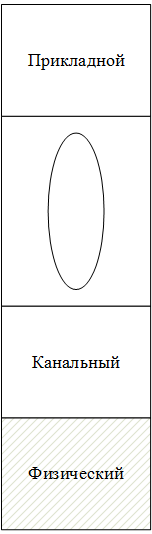
\includegraphics[width=0.2\linewidth]{img/system_levels_LoRa}
	\caption{Разбиение на уровни системы LoRa}
	\label{fig:system_levels_LoRa}
\end{figure}
\subsubsection{Особенности построения уровней}
Физический уровень системы имеет специфические особенности, так как в нем используется специальная модуляция, называемая LoRa. Модули физического уровня системы являются закрытыми.

\newpage
	% !TeX spellcheck = ru_RU
% !TeX encoding = UTF-8
\section{Технология «СТРИЖ»}
\subsubsection{Назначение}
«СТРИЖ» — это беспроводная система сбора, передачи и обработки данных счетчиков, датчиков и приборов учета для ЖКХ, электроэнергетики и систем безопасности.

«СТРИЖ Телематика» разрабатывает и продвигает новый класс устройств, работающих по стандарту LPWAN (Low-Power Wide-Area Network). Эти устройства могут автономно работать на одной батарейке многие годы, передавая сигнал по радиоканалу на большие расстояния. 


К настоящему времени компания разработала и начала внедрение несколько типов устройств, которые используются для передачи данных в различных областях. В секторе ЖКХ — это счетчики воды и электричества, передающие показания, а также модемы для передачи показаний счетчиков воды, газа, электричества и тепла. Для сферы сельского хозяйства выпущены датчики влажности почвы для открытых полей большой площади и закрытых теплиц, термоштанга для контроля сохранности урожая через мониторинг температуры и датчик углекислого газа для контроля сохранности урожая через мониторинг концентрации диоксида углерода. В процессе разработки находится серия интегрированных устройств для учета тепла и охраны банкоматов.

\subsubsection{Структура системы}
Рассмотрим структуру системы «СТРИЖ». Типичная сеть «СТРИЖ» состоит из следующих элементов: 
\begin{itemize}
	\item"Датчики". Специальные устройства для сбора данных, изготовленные компанией «СТРИЖ Телематика».  
	\item"Приёмники". В технологии «СТРИЖ» используется термин "Базовая станция".
	\item"Пункт сбора". В технологии «СТРИЖ» используется термин "сервер «СТРИЖ»".
	\item Облачный сервер. С сервера «СТРИЖ» данные передаются либо в личный кабинет пользователя "в облаке", либо на сервер клиента.
\end{itemize}
Структурная схема системы представлена на рисунке
\ref{fig:Swift}.

\begin{figure}[H]
	\centering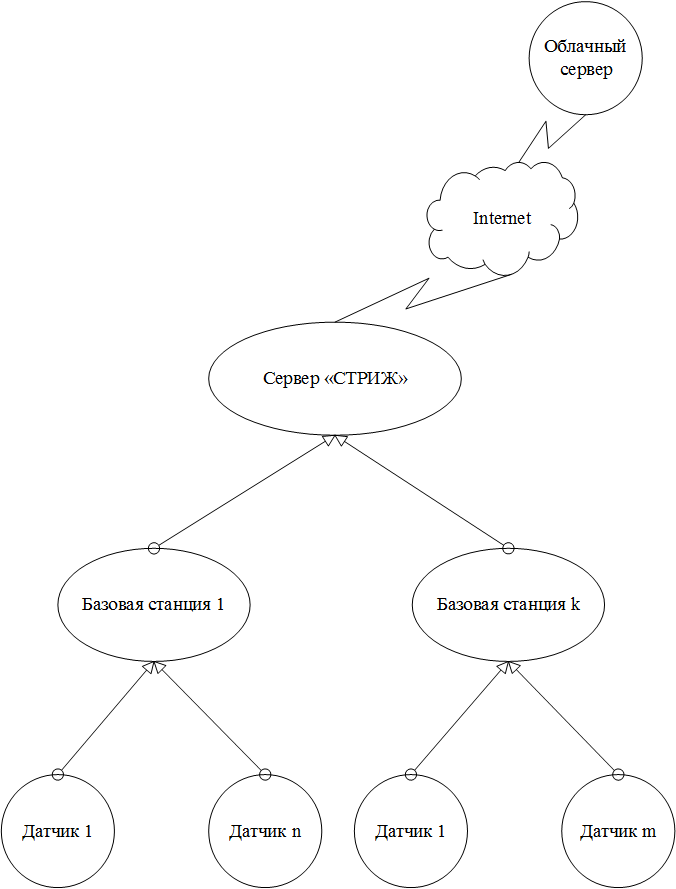
\includegraphics[width=0.7\linewidth]{img/Swift}
	\caption{Структурная схема системы, построенной по технологии «СТРИЖ»}
	\label{fig:Swift}
\end{figure}

Подход, используемый для передачи данных в сети «СТРИЖ», очень похож на принцип работы сотовых сетей.

Устройства «СТРИЖ» передают показания в личный кабинет клиента через базовую станцию, где они обрабатываются и предоставляются в удобном для пользователя виде. Обратный канал позволяет управлять отдельными приборами удаленно\cite{2}.

Однако, в отличие от технологии мобильной связи, «СТРИЖ» использует свой энергоэффективный радиопротокол, что позволяет передавать данные на расстояния до 50 км и обеспечить автономность работы устройств свыше 10 лет без внешнего питания.


\subsubsection{Разбиение системы на уровни}

Способ разбиения системы «СТРИЖ» на уровни представлен на рисунке
\ref{fig:system_levels_1}.
\begin{figure}[H]
	\centering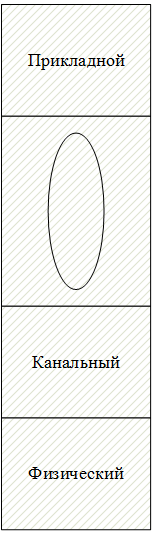
\includegraphics[width=0.2\linewidth]{img/system_levels_1}
	\caption{Разбиение на уровни системы «СТРИЖ»}
	\label{fig:system_levels_1}
\end{figure}

\subsubsection{Особенности построения уровней}
Главной особенностью построения уровней системы «СТРИЖ» является то, что все уровни данной системы являются закрытыми.
 
Особенностью физического уровня системы можно считать то, что устройства и модемы «СТРИЖ» не требуют подключения к электросети. Они вообще не требовательны к питанию. Процесс отправки данных оптимизирован, а мощность передачи в 80 раз ниже, чем у мобильного телефона. Именно поэтому одного источника питания хватает на 10 лет работы прибора.\newpage
	% !TeX spellcheck = ru_RU
% !TeX encoding = UTF-8
\section{Технология Lonta Optima}
\subsubsection{Назначение}
Радиоканальная система пультовой охраны Lonta Optima компании «Альтоника» предназначена для централизованной охраны территориально распределенных стационарных объектов с передачей охранно-пожарных извещений по радиоканалу.
\subsubsection{Структура системы}
Рассмотрим структуру системы Lonta Optima. Типичная сеть Lonta Optima состоит из следующих элементов: 
\begin{itemize}
	\item"Датчики". В технологии Lonta Optima "датчиками" являются приемно-контрольные приборы со встроенным передатчиком.  
	\item"Приёмники". В технологии  Lonta Optima используется термин "выносной приемник".
	\item"Пункт сбора". В технологии  Lonta Optima "пунктом сбора" является пульт централизованного наблюдения. В большинстве случаев пульт централизованного наблюдения подключается к компьютеру с программным обеспечением рабочего места оператора(по полученным данным производится охранный мониторинг), но может использоваться и автономно.  
\end{itemize}

Структурная схема системы представлена на рисунке
\ref{fig:Lonta_Optima}.

\begin{figure}[H]
	\centering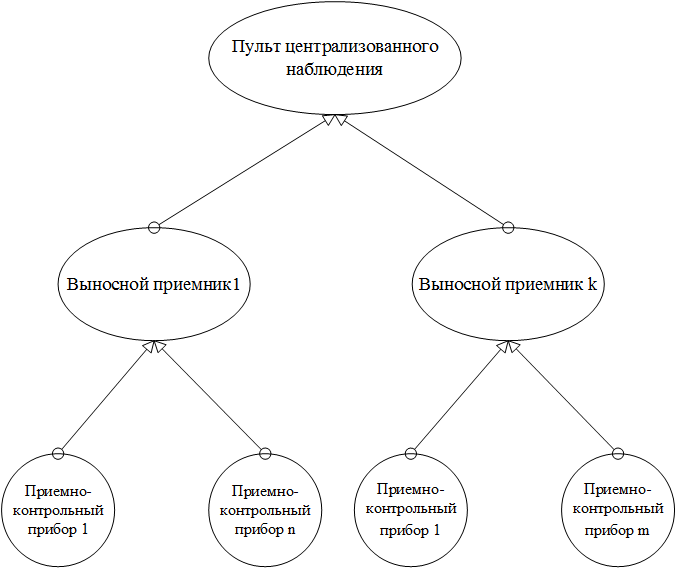
\includegraphics[width=0.7\linewidth]{img/Lonta_Optima}
	\caption{Структурная схема системы, построенной по технологии Lonta Optima}
	\label{fig:Lonta_Optima}
\end{figure}

В состав системы с одним пультом может входить до 500 передатчиков.

В системе Lonta Optima базовая станция и передатчики работают на определенном наборе частот в пределах разрешенной полосы 433,92 МГц. Этот набор частот называется «частотная литера». Всего в разрешенной полосе частот можно при необходимости разместить до 36 неперекрывающихся литер.
В одном городе или районе на разных частотных литерах одновременно могут работать до четырех систем Lonta Optima.

\textbf{Особенности:}
\begin{itemize}

\item Дальность связи составляет до 10 км в условиях городской застройки и до 25 км за городом.
\item Контроль связи с каждым объектом - 20-90 минут (устанавливается пользователем).
\item На одной территории возможно одновременное использование 2000 передатчиков на 4 частотных литерах.
\end{itemize}

\subsubsection{Разбиение системы на уровни}
Способ разбиения системы  Lonta Optima на уровни представлен на рисунке
\ref{fig:system_levels}.
\begin{figure}[H]
	\centering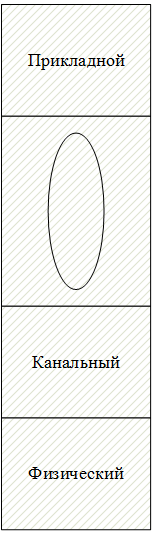
\includegraphics[width=0.2\linewidth]{img/system_levels}
	\caption{Разбиение на уровни системы Lonta Optima}
	\label{fig:system_levels}
\end{figure}

\subsubsection{Особенности построения уровней}
Главной особенностью построения уровней системы  Lonta Optima является то, что все уровни данной системы являются закрытыми.

\textbf{Особенности физического уровня системы:}

\begin{itemize}
	
	\item Для эксплуатации системы не требуется получение разрешения на использование радиочастоты.
	\item Система работает на открытой частоте 433,92 МГц.
	\item Мощность объектовых передатчиков составляет 10 мВт\cite{3}.
	
\end{itemize}

\newpage\newpage
	% !TeX spellcheck = ru_RU
% !TeX encoding = UTF-8
\section{Технология SigFox}
\subsection{Назначение системы}
Компания \textbf{Sigfox} (Франция) занимается разработкой и внедрением технологии сверх узкополосной (\textbf{UNB} — Ultra Narrow Band) беспроводной связи для передачи данных в субгигагерцовом нелицензируемом диапазоне 868.8 MГц. Сеть компаний развернута в Европе: Франция, Италия, Великобритания, Ирландия, Испания, Португалия, Люксембург, Нидерланды, Бельгия, Дания. 

Основная разработка Sigfox — энергоэкономные беспроводные сети, которые станут основой интернета вещей. Благодаря этим сетям между собой смогут обмениваться данными «умные» часы, телевизоры, микроволновые печи, стиральные машины и другие устройства. Эта технология изначально предназначена для связи на низких скоростях передачи данных. SigFox в настоящее время использует самый популярный европейский \textbf{ISM} диапазон на 868 МГц (как определено стандартом ETSI и СЕРТ), а также 902 МГц в США (как определено FCC), в зависимости от конкретных региональных правил. Система развернута с использованием возможностей современных сотовых сетей.
\subsection{Структура системы}
Устройство может отправить до 140 сообщений в день, и каждое сообщение может содержать до 12 байт полезных данных. 12 байт покрывает потребности устройств, которые передают данные, такие как местоположение устройства, индекс потребления энергии, сигнал тревоги или любой другой тип основной сенсорной информации. 
Также можно передавать до 4 сообщений из 8 байт полезных данных на каждое устройство в сутки. Для того, чтобы получать сообщения, устройство должно запросить данные с сервера, это должно быть запрограммировано на конкретные события или на определенное время, что позволяет экономить энергию, находясь большую часть времени в спящем режиме. 8 байт, отправленные на устройство, позволяют при необходимости отправить данные конфигурации, можно оптимизировать срок службы аккумулятора. Этого достаточно, если нет необходимости в полноценной двусторонней связи. На данный момент система Sigfox реализована с односторонней связью: данные с датчиков агрегируются и передаются на сервера компании Sigfox(\ref{fig:img11}). 
\begin{figure}[H]
	\centering
	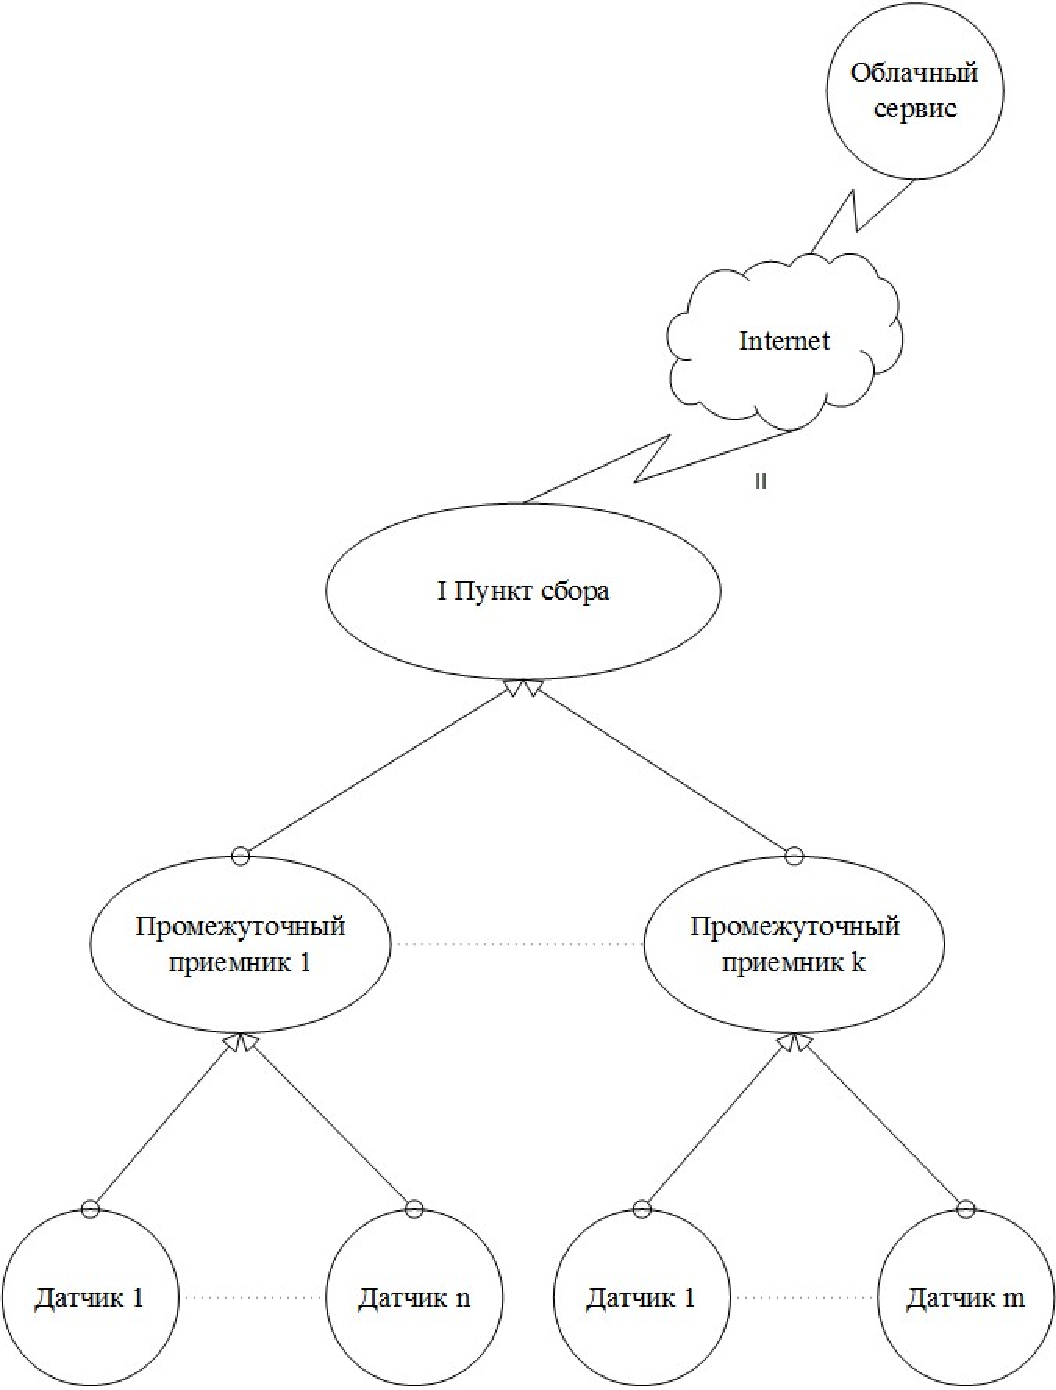
\includegraphics[width=0.5\textwidth]{img/kich_bur/11.pdf}
	\caption{Стурктура системы Sigfox}
	\label{fig:img11}
\end{figure}
\subsection{Разбиение системы на уровни}
Sigfox — исторически первая крупная компания на рынке интернета вещей — выбрала для себя довольно закрытую модель. На рисунке \ref{fig:img12} представлено разбиение системы на уровни. У Sigfox необходимо купить базовые станции и заключить с ним договор на разворачивание сети, к которой будет предоставляться платный доступ сторонним абонентам. Базовые станции передают данные на сервера Sigfox, то есть канал связи --- не физический, но логический и ПО верхнего уровня также принадлежат Sigfox. Sigfox не стал узурпировать рынок чипов и конечных устройств --- он договорился с Texas Instruments, SiLabs и другими производителями о поддержке своей сети, что позволяет заказать какое-то нестандартное Sigfox-устройство. К сожалению, проблему может составить его подключение к сети: если в Европе Sigfox успел развернуться, то сейчас, с появлением LoRa, его экспансия фактически остановилась.
Сотовые сети LPWAN --- сети масштаба городов --- это сети с множеством базовых
станций (например, на покрытие Москвы надо порядка 200 штук), как правило, обслуживаемые оператором сети, предоставляющим за деньги доступ к ней владельцам конечных устройств. Sigfox устанавливает жесткую тарифную сетку. 
\begin{figure}[H]
	\centering
	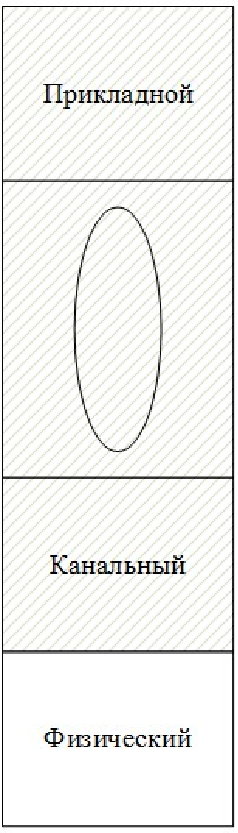
\includegraphics[width=0.2\textwidth]{img/kich_bur/12.pdf}
	\caption{Разбиение системы Sigfox на уровни}
	\label{fig:img12}
\end{figure}
Таким образом, все уровни закрыты, за исключением физического, что позволяет
сделать гибкую сетку маломощных устройств. 
\subsection{Особенности построения уровней}
Sigfox не поддерживает топологию «звезда». Ни в Sigfox, ни в «Стриже», ни вообще в мире узкополосных UNB-систем сети такой топологии технически невозможны: из-за специфики UNB-систем абонентское устройство в общем случае не может принимать данные в произвольные моменты времени от других абонентских устройств, а значит, не может выступать в качестве ретранслятора.
Все решения распадаются на две группы: широкополосные UWB (Ultra Wide Band, к ним из перечисленного относится только LoRa) и узкополосные UNB (Ultra Narrow Band, в нашем случае это Sigfox и «Стриж»). Из этого проистекает ряд отличий.
UWB: один канал занимает полосу в эфире с шириной 125 или 250 кГц
UNB: один канал занимает полосу в эфире с шириной 100 Гц

В России в диапазоне, условно именуемом «\textbf{868 МГц}», для
неспециализированных устройств официально доступны две полосы частот:
864,0-865,0 МГц с периодом активной работы не более одной десятой процента и
запретом на работу вблизи аэропортов и 868,7-869,2 МГц без таких ограничений. В общем случае мы имеем всего лишь 500 кГц доступной нам полосы частот. Каналов Sigfox при ширине 125 кГц в эту полосу умещаются сотни.

В UNB-системах один приёмник базовой станции в один момент времени может принимать только один канал.  Термин «частотное разделение» относится к способности приёмника выцепить этот канал из общего эфира так, чтобы на него не накладывалась передача в соседних каналах — и если мы в данную секунду принимаем что-то по каналу N, то по каналам N+1 и N-1 мы принять в это же время ничего не можем. В UWB-системах используется не только частотное и временное, но и кодовое разделение каналов.  

Из-за допплеровского эффекта Sigfox теряет стабильность работы уже на скорости движения конечного устройства в районе 5-10 км/ч. 

UNB-системы работают на фиксированной низкой скорости. У Sigfox скорость передачи данных 100 бит/с, у «Стрижа» — 50 бит/с.

Дальность связи во всех подобных технологиях очень сильно зависит от условий на местности: в целом можно считать, что все перечисленные технологии обеспечивают дальность 1-3 км в городской застройке и 15-20 км на открытой местности. Дальность может быть увеличена за счёт выгодного расположения антенн: например, слова «в городской застройке» могут означать как абонентские устройства, расположенные в глубине зданий и оснащённые компактными печатными антеннами, так и управляемые уличные фонари с обычными штыревыми антеннами, стоящими на открытом воздухе и минимум в пяти метрах от земли.
Энергопотребление сверхнизкое, по оценкам до 20 лет работы сенсора от 2-х батарей АА. 

\newpage\newpage
	% !TeX spellcheck = ru_RU
% !TeX encoding = UTF-8
\section{Сравнение систем}
Результаты сравнения систем представлены в таблице \ref{tab:table1}. 
\begin{table}
	\centering
	\resizebox{\textwidth}{!}{%
		\begin{tabular}{|p{3cm}|p{3cm}|p{3cm}|p{3cm}|p{3cm}|}\hline
			\begin{center}
				\textbf{Критерий сравнения системы }
			\end{center}&\begin{center}
			\textbf{LoRa}
		\end{center}&\begin{center}
		\textbf{«СТРИЖ»}
	\end{center}&\begin{center}
	\textbf{Lonta Optima} 
\end{center}&\begin{center}
\textbf{SigFox} 
\end{center}
                                            \\ \hline
			Возможность передачи от приёмников к датчикам&\begin{center}
				есть
			\end{center}&\begin{center}
			нет
		\end{center}&\begin{center}
		нет
	\end{center}&\begin{center}
		нет
	\end{center}\\ \hline 

			Скорость передачи данных от датчиков к приемникам&\begin{center}
				50 Кбит/с
			\end{center}&\begin{center}
			 50 бит/с
		\end{center}&\begin{center}
		 50 бит/с
	\end{center}&\begin{center}
		    10 - 100 бит/с\end{center}\\ \hline
			Дальность действия &до 5 км в условиях городской застройки и до 15 км в сельской местности&до 10 км в условиях городской застройки и до 50 км в сельской местности&до 10 км в условиях городской застройки и до 25 км в сельской местности&до 10 км в условиях городской застройки и до 50 км в сельской местности\\ \hline 
		\end{tabular}}
\end{table}
\newpage
\begin{table}
	\centering
	\resizebox{\textwidth}{!}{%
		\begin{tabular}{|p{3cm}|p{3cm}|p{3cm}|p{3cm}|p{3cm}|}\hline
Частотный диапазон&868-869 МГц (в Европе) &2,4 ГГц, 868/915 МГц, 433 МГц &433 МГц & 864-865 МГц, 868-869 МГц\\ \hline 
Открытые уровни&от канального уровня до прикладного уровня &все уровни являются закрытыми&все уровни являются закрытыми& физический уровень\\ \hline 
Закрытые уровни&физический уровень&все уровни являются закрытыми&все уровни являются закрытыми&от канального уровня до прикладного уровня\\
\hline 

  \begin{center}
  	 Стандарт
  \end{center}&\begin{center}
	LoRaWAN
\end{center}&\begin{center}
нет
\end{center}&\begin{center}
нет
\end{center}&\begin{center}
нет
\end{center}\\ \hline
\end{tabular}}
\caption{Результаты сравнения систем}.
\label{tab:table1}
\end{table}
\newpage
	\addcontentsline{toc}{subsection}{Список использованных источников}
	\begin{thebibliography}
		{1} \bibitem{1}\emph{}Описание технологии LoRa:
		
		\url{https://habrahabr.ru/company/rtl-service/blog/304312/}. 
		{2} \bibitem{2}\emph{}Официальный сайт компании «СТРИЖ Телематика»:
		
		\url{https://strij.tech}.
		{3} \bibitem{3}\emph{}Официальный сайт компании «Альтоника»:
		
		\url{http://www.altonika-sb.ru/}.   
	\end{thebibliography}
\end{document}